\section{Design Options}

In order to be able to register as a \acs{pci} device driver, some sort of
management process for receiving the interrupts is necessary. A management
process is also useful for device detection and initialization, providing the
system with an overall view of what devices are available.

Consumers of \ac{ahci}-related interrupts must register with the management
process so that interrupts may be forwarded. To provide clients with access to
different \ac{sata} devices, it makes sense to grant access to invidual
\ac{hba} ports, and similarly to forward all interrupts for a port to any
clients registered to that port.

However, in choosing the method of accessing the ports, a trade-off must be
made between security and performance. For example, by setting a suitable
address, another domain's memory can be written to disk, and then read back,
violating domain separation. To stop this from occuring, a central location
must check that all \acp{prd} reference memory which the client may access.

In such a design, all port memory access, including issuing of commands, would
happen via Flounder messages to the central daemon. The central daemon would
have to ensure that the client does not modify the command list or command
tables after they are checked, so the all these areas would have to be copied
into a memory area not accessible to the client.

To achieve optimal performance at the cost of security, each client must be
given full access to the port memory. Because this is usually within the same
page as the \ac{hba} memory, clients are able to access not just their own
port's registers, but all other ports' and the \ac{hba}'s registers as well.
Also, as described above, the client can access all memory with suitable
\acs{dma} commands.

\section{General Architecture}

\begin{figure}[ht]
\centering
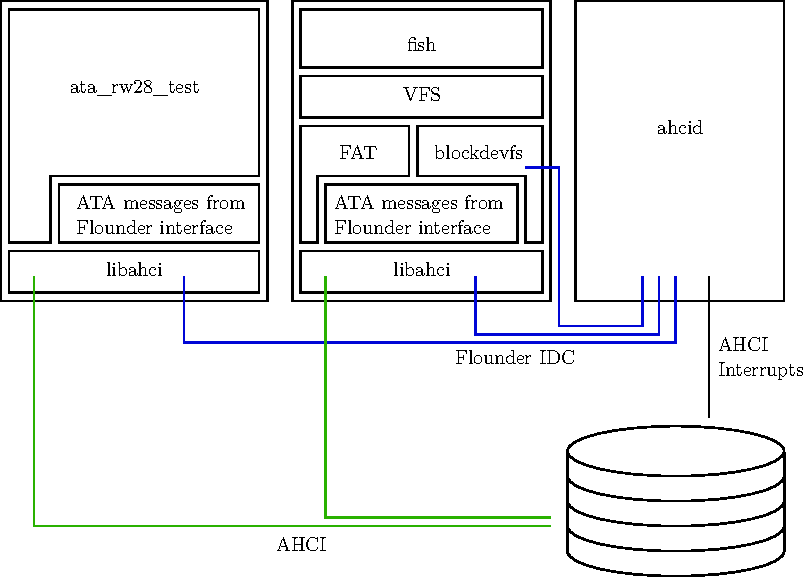
\includegraphics[width=.9\textwidth]{architecture.pdf}
\captionof{figure}{Barrelfish AHCI subsystem architecture}
\label{fig:architecture}
\end{figure}

As shown in in \autoref{fig:architecture}, our message passing to disk has two
main parts: a management part and a communication part. The management part,
\emph{ahcid}, provides a system-wide authority over an \ac{ahci} controller.
The communication part, consisting of libahci (a low-level abstraction for
using an \ac{ahci} port) and the \ac{ata} message specification and translation
layer using Flounder, is used by all user-level code that wants to access a
disk to send and receive messages from a disk.

\section{ahcid}

ahcid exists as a central point of authority over an \ac{ahci} \ac{hba}. It is
responsible for \ac{hba} initialization, Interrupt handling and access
mediation.

\subsection{Operation}

ahcid ensures only one user can access an \ac{ahci} port at a time. Users can
open a port by sending an \acs{idc} message to ahcid. If no other user
currently owns the port, ahcid will provide a memory capability to the port's
memory registers.  The user is then able to use the port exclusively.
Interrupts generated by the port are handled by ahcid and dispatched to the
associated user via an \acs{idc} message. ahcid registers itself as PCI device
driver for certain \ac{ahci} chipsets.

\section{libahci}

libahci tries to hide the necessary bit-twiddling and \acs{dma} buffer
management for sending and receiving messages to a disk. Its interface
resembles a Flounder-generated interface and makes use of Barrelfish's
waitsets.

\section{Flounder Backend}

This lab project also contains a Flounder backend and Flounder modifications in
order to be able to specify \ac{ata} commands as message definitions. The
resulting interface can be used similarly to performing \acs{idc}.

\section{Implemented ATA Commands}

For our purposes (designing a messaging interface to disks) it was sufficient
to implement commands for reading and writing blocks to and from disks using
\acs{dma} (\ac{ata} commands {\tt READ DMA}, {\tt WRITE DMA}), inspecting the
disk ({\tt IDENTIFY}) and flushing the cache ({\tt FLUSH CACHE}). Due to the
Flounder layer in our system (specifically the \acs{ahci} backend) adding new
\ac{ata} commands is quite easy: just add the command you want in the \ac{ata}
interface specification.
